\chapter{Lernskript}
\section{Enum-Klasse}
 \begin{lstlisting}[language=JAVA]
enum Color {Red, Green, Blue, Yellow}
\end{lstlisting}
in etwa äquivalent zu
\begin{lstlisting}[language=JAVA]
class Color
{
	final static Color Red      = new Color();
	final static Color Green  = new Color();
	final static Color Blue     = new Color();
	final static Color Yellow = new Color();
}
\end{lstlisting}
\begin{itemize}
        \item Gleich benannte Enumwerte in unterschiedlichen Enumtypen sind inkompatibel
	\item Enum-Literal = enumtype.enumelement
	\item Definition  einer Variablen
 \begin{lstlisting}[language=JAVA]
       Color c;
	c = Color.Red;
	if (c == Color.Yellow) ...
	\end{lstlisting}
	\item Enumtypen = Referenztypen, Enumwerte = Klassenvariablen
	\item Vordefinierte Methoden in allen Enumtypen E:
	\begin{itemize}
		\item static E valueOf(String s) = Enumwert mit dem Namen s
		\item static E[] values () = Array mit allen Enumelementen
	\end{itemize}
	\item Begriffe Enumelement = Enumwert = Enumobjekt
	\begin{itemize}
	\item Enumobjekte sind eindeutig
	\item zusätzliche Objekte können nicht erzeugt werden, 
	\item Vergleich mit == statt equals ausreichend
	\end{itemize}
\end{itemize}
%
%
%
\section{Unified Modelling Language (UML)}
\subsection{Basics}
\begin{figure}[H]
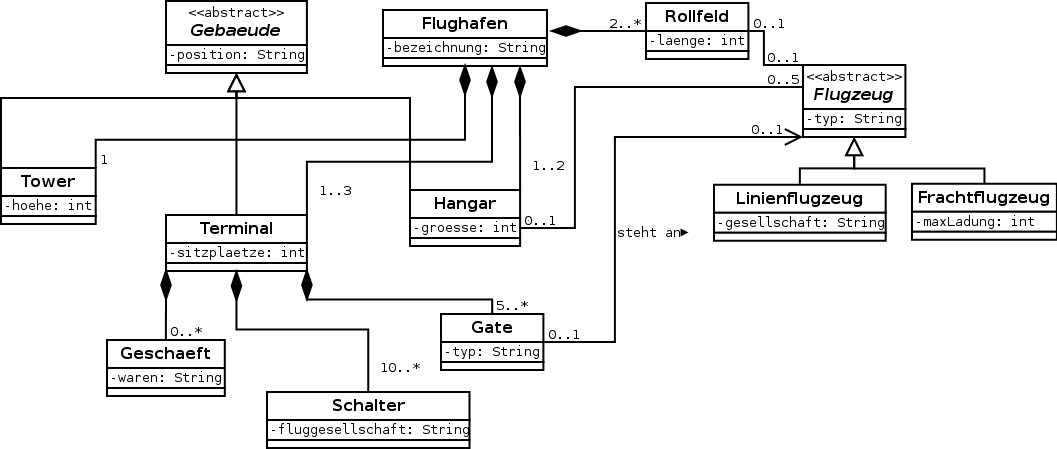
\includegraphics[width=15cm]{mainmatter/pics/Flughafen.png}
\end{figure}

\subsection{Interfaces}
\begin{figure}[H]
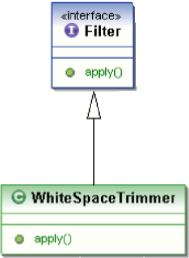
\includegraphics[width=4cm]{mainmatter/pics/interfaces.png}
\end{figure}

\subsection{Objektdiagramme}
\begin{figure}[H]
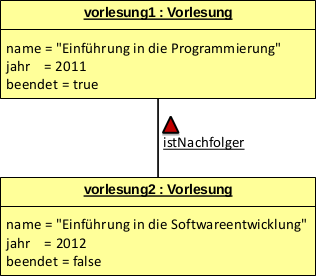
\includegraphics[width=6cm]{mainmatter/pics/objektdiagramm.png}
\end{figure}
\begin{figure}[H]
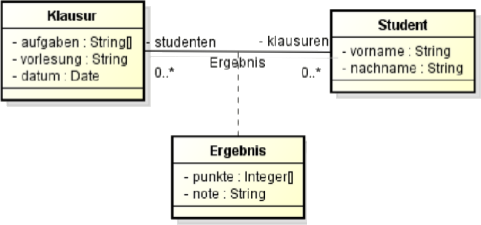
\includegraphics[width=6cm]{mainmatter/pics/zwischending.png}
\end{figure}
 %
 %
 %
 \section{Design Pattern}
\subsection{Observer-Pattern}

\subsection{Decorator-Pattern}
„Decorator fügt einem Objekt dynamisch zusätzliche Verantwortlichkeiten hinzu. Dekorierer bieten eine flexible Alternative zur Ableitung von Unterklassen zum Zweck der Erweiterung der Funktionalität“

\begin{itemize}
	\item Vorteile:
	\begin{itemize}
\item Sehr flexibel und mächtig
\item Sehr dynamisch – Dekorationen können zur Laufzeit geändert werden
\item Basisklasse (Komponente, Eis, InputStream) muss zur Anwendung des Patterns nicht geändert werden!
\item Decorator können um bereits bestehende Klassen gelegt werden, ohne diese zu modifizieren!
\item Dekoratoren sind für Client-Code völlig transparent – sie können wie die ursprüngliche Klasse verwendet werden
\item Führt zu flachen Vererbungshierarchien
	\end{itemize}
	\item Nachteile:
	\begin{itemize}
\item Fehler zu finden ist in langen Decorator-Ketten oft schwierig
\item API wird schnell durch viele kleine Objekte aufgebläht und schwer verständlich
\item Direkte Erstellung dekorierter Klassen ist umständlich (dafür gibt es aber auch wieder Pattern...)
\item  Sinnlose oder gefährliche Kombinationen von Decorators können nur schwer verhindert werden
\item Decorator ist nicht angebracht, falls genaue Informationen über die Typen und Anzahlen von Dekorationen benötigt werden
	\end{itemize}
\end{itemize}
%
%
%
\section{Wrapperklassen}
\begin{tabular}{|l|l|}
\textbf{Primitiver Typ} & \textbf{Wrapper-KLasse}\\\hline
byte & Byte \\\hline
short & Short \\\hline
int & Integer \\\hline
long & Long \\\hline
double & Double \\\hline
float & Float \\\hline
char & Character \\\hline
void & Void \\\hline
\end{tabular}
Wrapper-Objekte können auf drei Arten entstehen:
\begin{itemize}
\item Durch Aufruf einer statischen valueOf()-Methode der Wrapper-Klasse, der ein primitiver Ausdruck oder ein String übergeben wird
\item Durch Boxing: für primitive Werte erzeugt der Compiler automatisch valueOf()-Methodenaufrufe, die eine Instanz der Wrapper-Klasse zurückliefern
\item Durch Aufruf von new und die Konstruktoren der Wrapper-Klassen
\end{itemize}

\begin{lstlisting}[language=JAVA]
Integer i = Integer.valueOf("42"); // statische valueOf()-Methode
Long l = new Long(123); 		// Konstruktoraufruf
Double d = 12.3;				// Boxing
//
//
Integer int_wrap_array[] = {1, 2, 3}; // Ok ueber Boxing
int int_array[] = int_wrap_array; // Fehler!
int i = int_wrap_array[0]; // Ok ueber Unboxing
//
//
Integer i = 42;
i = i +1 // Integer hat kein + Unboxing

Integer j = 42;
if (i==j) {...} // == auf Integer moeglich: kein Unboxing !Vergleich auf Identitaet! 
//Daher Fehler
\end{lstlisting}
\section{Collections}
\begin{itemize}
\item Java bietet eine Klassenhierachie für dynamsiche Container an, die sogenannten Collections
\item Collections sollen zwar Objekte beliebiger Klassen speicher können, müssen dabei aber typsicher sein
\item In jede Collection "passt" jeweils nur ein Typ von Objekten (bzw. natürlcih auch alle Instanzen von ihm abgeleiteter Typen)
\item nur durch Generics möglich
\end{itemize}
\section{Generics}
\begin{description}
	\item[Beobachtung:] oft ist die Formulierung einer bestimmten Klasse oder die Arbeitsweise eines bestimmten Algorithmus unabhängig von den exakten beteiligten Typen
	\item[Beispiele:]
	\begin{itemize}
		\item Container sind Klassen zum Speichern meherer Objekte als Elemente. Der Aufbau des Containers ist oft unabhängig vom gespeicherten Typ, dieser muss aber zur Implementierung angegeben werden
		\item Sortieralgorithmen werden üblicherweise unabhängig vom zu sortieren Typ entwickelt wobei dei Existenz einer Vergelcihsfunktion bekannten Namens für dne Typ vorausgesetzt wird. Zur Implementierung des Algorithmus muss aber ein konkreter Typ angegeben werden.
	\end{itemize}
\end{description}
\begin{itemize}
	\item Generics = Platzhalter 
	\begin{lstlisting}[language=JAVA]
class Node<T>
{
private T info;
private Node<T> left;
private Node<T> right;
}
\end{lstlisting}
	\item Generics mit Restriktionen
	\begin{lstlisting}[language=JAVA]
	class Node<T extends Number>
	\end{lstlisting}

\item Kompatibilität zwischen Typen 
	\begin{itemize}
	\item Implizite Typkonversion \\ für bestimmte primitive Typen (nicht für Arrays)
	\begin{lstlisting}[language=JAVA]
	int i = 1; double d  =i;
	\end{lstlisting}
\item Implementierung\\
Klasse => Interface (einschließlich arrays)
	\begin{lstlisting}[language=JAVA]
	Cartesian ct = new Cartesian(1,2); Complex cx = ct;
	\end{lstlisting}
\item Vererbung \\ Abgeleitete KLasse => Basisklasse (einschließlich Arrays)
	\begin{lstlisting}[language=JAVA]
	String s = "foo", Object o = s;
	\end{lstlisting}
\item Autoboxing \\ Primitiver Typ => Wrapperklasse (nicht für Arrays)
	\begin{lstlisting}[language=JAVA]
	int i = 1; Integer it = i;
	\end{lstlisting}
\item Auto-Unboxing \\ Wrapperklasse => primitiver Typ (nicht für Arrays)
	\begin{lstlisting}[language=JAVA]
	Integer it = new Integer(2); int i = it;
	\end{lstlisting}
\end{itemize}
\item Generic Invarianz
\begin{lstlisting}[language=JAVA]
Node<Number> nn = new Node<Integer>(23); /7 Fehler
\end{lstlisting}
\item Generic Wildcartypen
\begin{lstlisting}[language=Java]
Node<?> nx
//=============================
nx = new Node<?>(); // Fehler
//=============================
Node<?> nx;
nx = new Node<String>("foo");// ok
nx = new Node<Integer>(1);// ok
nx = new Node<Double>(3.14);// ok
\end{lstlisting}
\item Mögliche Varianzen \\
\begin{tabular}{|l|l|l|l|l|}\hline
\textbf{Varianz} & \textbf{Syntax} & \textbf{Lesen}  & \textbf{Schreiben} & \textbf{Typargumente} \\ 
&&&&\textbf{kompatibler Typen} \\\hline
Invarianz & C<T> & erlaubt & erlaubt & T\\\hline
Bivarianz & C<?> & verboten & verboten & alle \\\hline
Covarianz & C<? extend B> & erlaubt & verboten & B und abgeleitete Typen \\\hline
Contravarianz & C<? super B> & verboten & erlaubt & B und Basistypen\\\hline 
\end{tabular}
\end{itemize}
%
%
%
\section{Kontrollflussgraph}
\begin{figure}[H]
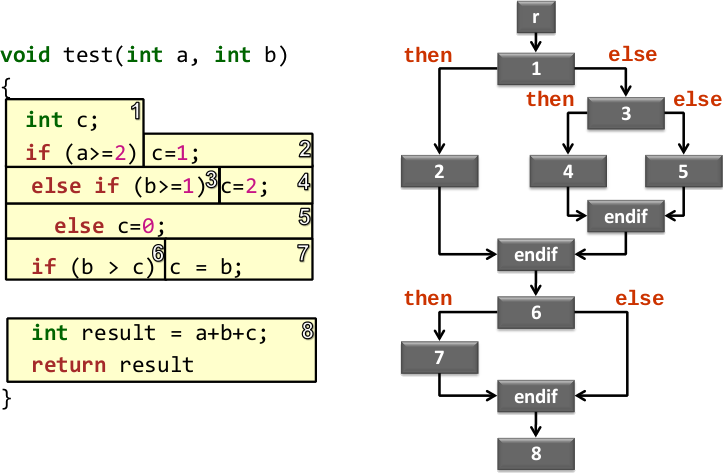
\includegraphics[width = 10cm]{mainmatter/pics/Kontrollflussgraph.png}
\end{figure}
%
%
%
\section{Testfälle}
\begin{itemize}
\item Testfall C$_{0}$ \\ Finde Testfälle, durch die alle Knoten des Kontrollflussgraphen einmal besucht werden! \\ Anweisungsüberdeckung
\item Testfall C$_{1}$ \\ Finde Testfälle, durch die alle Kanten des Kontrollflussgraphen einmal verwendet werden! \\ Zweigüberdeckung
\item Testfall C$_{2}$ \\ Finde Testfälle, die zusammen alle Pfade durch den Kontrollflussgraphen durchlaufen \\ Pfadüberdeckung 
\item Testfall C$_{2}$b \\ teste alle Pfade, aber bei Schleifen nur "durchlaufen" und "übersprungen"
\item Testfall C$_{2}$c \\ teste alle PFade aber Schleifen nur bis n $\in \mathbb{N}$ Durchläufen
\item Testfall C$_{3}$ \\ Finde Testfälle, die alle Bedingungen des Programms testen! \\ Bedingungsüberdeckung 
\item Testfall C$_{3}$a \\ Jede atomare Bedinung soll einmal true und einmal false annehmen
\item Testfall C$_{3}$b \\ jede Kombination atomarer Bedingungen soll getestet werden.
\item Testfall C$_{3}$c \\ jede atomare Bedingung und jede kombinierte Bedingung soll einaml true und einmal falls annehmen
%
%
%
\section{Testen mit JUnit}
Annotationen:
\begin{itemize}
\item @Test\\Testmethode (kann mehrfach vorkommen)
\item @Before \\ Wird vor jedem einzelnen Test aufgerufen
\item @After \\ Wird nach jedem einzelnen Test aufgerufen
\item @BeforeClass \\ Wird einmal vor allen Tests aufgerufen
\item @AfterClass \\ Wird einmal nach allen Tests aufgerufen
\item Testfall für gcd(1,1) = :\\
\begin{lstlisting}[language=JAVA]
@Test public void test11()
{
	int want = 1
	int have = new GCD().gcd(1,1);
	assertEquals(want,have)
}
\end{lstlisting}
\item Test mit Exception Erwartung \\
\begin{lstlisting}[language=JAVA]
@Test(expected=ArithmeticException.class)
public void test10()
{...}
\end{lstlisting}
\end{itemize}
%
%
%
\section{GUI}
\section{Threads}